\documentclass[twocolumn]{aastex631}

\usepackage{amsmath}
\usepackage{multirow}
\usepackage{natbib}
\usepackage{graphicx} 
\usepackage{aas_macros}


\begin{document}

\title{Field-Dependent Symmetries for One-Loop Ghost-Free Type I DHOST Theories: A Cosmological Confrontation}

\author{Denario}
\affiliation{Anthropic, Gemini \& OpenAI servers. Planet Earth.}

\begin{abstract}
Higher-derivative scalar-tensor theories are prone to Ostrogradsky ghost instabilities. While Degenerate Higher-Order Scalar-Tensor (DHOST) theories classically avoid these through kinetic degeneracy, quantum loop corrections can reintroduce them, posing a critical challenge to their viability. This work systematically identifies fundamental field-dependent symmetries in Type I DHOST theories with massless gravity in a Friedmann-Robertson-Walker background that ensure ghost-freedom at both tree-level and one-loop quantum levels. Using perturbation theory and one-loop effective action techniques, we first establish precise algebraic conditions for classical ghost-free scalar and tensor perturbations, including unity gravitational wave speed. We then derive and classify field-dependent symmetries that both leave the action invariant and structurally protect the kinetic degeneracy from quantum corrections. Our analysis identifies a specific class of shift-symmetric DHOST theories, characterized by a gravitational coupling proportional to the scalar field's kinetic term, possessing a hidden conformal symmetry that ensures robust quantum stability; an explicit one-loop calculation confirms the non-renormalization of the ghost kinetic term. A representative model from this quantum-stable class was tested against cosmological observations. While it reproduces a standard expansion history and predicts a gravitational slip parameter consistent with General Relativity, it catastrophically predicts a dramatically negative effective gravitational constant, implying repulsive gravity for matter and unequivocally ruling it out phenomenologically. This work provides a constructive framework for identifying quantum-stable modified gravity theories, highlighting the profound tension between theoretical robustness and observational viability.
\end{abstract}

\keywords{Cosmological perturbation theory, Observational cosmology, Large-scale structure of the universe, Accelerating universe, Gravitational waves}


\section{Introduction}
\label{sec:intro}

The standard cosmological model, $\Lambda$CDM, has achieved remarkable success in describing the Universe across vast scales and epochs, from the early Cosmic Microwave Background anisotropies to the formation of large-scale structures today. However, its foundation rests upon two enigmatic components: dark energy, posited to drive the Universe's accelerated expansion, and dark matter, which dominates the gravitational dynamics of galaxies and clusters. The unknown fundamental nature of these constituents motivates a critical exploration of alternative explanations, particularly through modifications to Einstein's theory of General Relativity (GR).

Scalar-tensor theories represent a broad and compelling class of modified gravity models where gravity is mediated not solely by the metric tensor, but also by a dynamical scalar field. These theories offer a potential avenue to address the dark energy problem, possibly providing a more fundamental description of cosmic acceleration without resorting to an exotic fluid. However, extending GR by introducing new degrees of freedom, especially those involving higher-order derivatives in the Lagrangian, frequently leads to severe theoretical pathologies. The most notorious of these is the Ostrogradsky instability, which manifests as a ghost—a field with negative kinetic energy—leading to runaway solutions and rendering the theory classically unstable.

To circumvent this fundamental problem, specific classes of higher-derivative scalar-tensor theories have been developed. Horndeski theories, the most general scalar-tensor theories yielding second-order field equations, are classically ghost-free by construction. Beyond Horndeski, Degenerate Higher-Order Scalar-Tensor (DHOST) theories extend this framework by allowing for Lagrangians with higher-order derivatives while ingeniously circumventing the Ostrogradsky instability at the classical (tree-level) by ensuring a kinetic degeneracy. This degeneracy effectively eliminates the problematic ghost degree of freedom, allowing the theory to propagate only the healthy tensor and scalar modes.

While classically ghost-free, the viability of DHOST theories faces a profound and more subtle challenge at the quantum level. It has been shown that quantum loop corrections can, in principle, reintroduce the very ghost that was classically removed by the kinetic degeneracy. The mechanism for this re-emergence involves the quantum integration out of healthy modes in loop diagrams, which can generate a non-degenerate kinetic term for the previously eliminated ghost, thereby destabilizing the theory at the quantum level. This re-emergence of the ghost at one-loop poses a critical barrier to the theoretical consistency and physical viability of DHOST theories, transforming a classically sound framework into a potentially pathological quantum field theory. The fundamental problem, therefore, lies in identifying DHOST theories that maintain their ghost-free nature not only at tree-level but also under quantum corrections. This is a difficult problem because the degeneracy condition, which ensures classical ghost-freedom, must be structurally protected from quantum fluctuations, requiring a deeper understanding of the theory's symmetries and their impact on its quantum effective action.

In this work, we undertake a systematic investigation into Type I DHOST theories with massless gravity in a Friedmann-Robertson-Walker (FRW) background, specifically aiming to resolve this critical quantum stability issue. Our central hypothesis is that specific, fundamental field-dependent symmetries can act as protective mechanisms, preserving the kinetic degeneracy structure against quantum radiative corrections. We propose a constructive framework to uncover and derive these symmetries from first principles.

Our approach begins by establishing the most general algebraic conditions on the DHOST functions, $G_i(\phi, X)$, that ensure tree-level ghost-freedom for both scalar and tensor perturbations. This includes the crucial requirement that gravitational waves propagate at the speed of light, i.e., $c_T^2=1$, and the condition for scalar degeneracy, $\mathcal{A}_S=0$. Subsequently, we delve into the intricate degeneracy structure of the DHOST Lagrangian and its quantum effective action. Here, we identify the precise properties that are essential to prevent the re-emergence of ghosts at the one-loop level, recognizing that a mere invariance of the action is insufficient; the symmetry must actively protect the underlying kinetic degeneracy. Building upon these insights, we systematically derive and classify the most general field-dependent symmetries—encompassing generalized shift and disformal transformations such as $\delta\phi = c$ and $\delta g_{\mu\nu} = \Omega(\phi, X) g_{\mu\nu} + \Gamma(\phi, X) \partial_\mu\phi \partial_\nu\phi$ for arbitrary functions $c, \Omega, \Gamma$—that not only leave the action invariant but also inherently satisfy the conditions for robust one-loop ghost stability. This systematic derivation yields a specific class of DHOST theories, characterized by particular functional forms of their gravitational couplings, which are demonstrably protected by these symmetries.

To verify our theoretical findings, we perform an explicit one-loop calculation for a representative model selected from our identified quantum-stable class. This calculation, employing the background field method, rigorously demonstrates how the derived symmetries ensure the non-renormalization of the ghost kinetic term, confirming its persistent absence at the quantum level. Finally, we confront these theoretically robust, quantum-stable theories with cosmological observations. We analyze their ability to reproduce a standard cosmological expansion history and examine their predictions for linear structure growth, specifically the effective gravitational constant $G_{\text{eff}}$ and the gravitational slip parameter $\eta$. This observational confrontation reveals a profound tension: while our framework successfully identifies a class of DHOST theories that are theoretically sound at the quantum level, a representative model from this class catastrophically predicts repulsive gravity for matter, unequivocally ruling it out phenomenologically. This work thus provides a powerful, constructive framework for identifying quantum-stable modified gravity theories, while simultaneously highlighting the formidable challenges in constructing models that are both theoretically robust and observationally viable.


\section{Methods}
\label{sec:methods}
Our methodological approach is designed to systematically identify and characterize Type I Degenerate Higher-Order Scalar-Tensor (DHOST) theories that are free from ghost instabilities at both tree-level and one-loop quantum levels, particularly within a cosmological Friedmann-Robertson-Walker (FRW) background. This involves a rigorous theoretical analysis, starting from the fundamental action, progressing through perturbation theory to establish classical stability, then deriving conditions for quantum stability, and finally confronting the resulting theories with cosmological observations.

\subsection{Theoretical Framework and Background Setup}
We begin by establishing the fundamental theoretical framework for our analysis. The master action for Type I DHOST theories, which encompasses Horndeski theories as a special case, is adopted in the form most convenient for our calculations. This action is expressed in terms of the functions $G_i(\phi, X)$, where $\phi$ is the scalar field and $X = -g^{\mu\nu}\partial_\mu\phi\partial_\nu\phi$ is its kinetic term. Specifically, the action is given by:
$$ S = \int d^4x \sqrt{-g} \left[ G_2(\phi, X) - G_3(\phi, X)\Box\phi + G_4(\phi, X)R - 2G_{4X}(\phi, X)((\Box\phi)^2 - \phi_{;\mu\nu}\phi^{;\mu\nu}) + G_5(\phi, X)G_{\mu\nu}\phi^{;\mu\nu} - \frac{G_{5X}(\phi,X)}{6}((\Box\phi)^3 - 3\Box\phi \phi_{;\mu\nu}\phi^{;\mu\nu} + 2\phi_{;\mu\nu}\phi^{;\nu\sigma}\phi_{;\sigma}^{\;\mu}) \right] $$
Here, $R$ is the Ricci scalar, $G_{\mu\nu}$ is the Einstein tensor, and $G_{iX} = \partial G_i / \partial X$. This formulation explicitly highlights the higher-derivative terms characteristic of DHOST theories.

For the cosmological analysis, we specialize to a flat Friedmann-Robertson-Walker (FRW) background, described by the metric $ds^2 = -dt^2 + a(t)^2 \delta_{ij} dx^i dx^j$, where $a(t)$ is the scale factor. In this background, the scalar field is assumed to be homogeneous, $\phi = \phi_0(t)$, which implies its kinetic term is $X = \dot{\phi}_0(t)^2$. All DHOST functions $G_i$ and their derivatives are evaluated on this homogeneous background solution. The background evolution of the Universe is governed by the two Friedmann equations, which are derived by varying the master action with respect to the metric components and evaluating the resulting equations on the FRW background with a homogeneous scalar field. These equations provide the foundational description of the Universe's expansion history within the context of DHOST theories.

\subsection{Tree-Level Stability Analysis and Degeneracy Conditions}
Ensuring classical stability is the next crucial step. This involves analyzing linear perturbations around the FRW background and imposing conditions that guarantee the absence of ghost and gradient instabilities.

\subsubsection{Perturbation Theory and Quadratic Action}
We introduce linear perturbations for both the metric and the scalar field around the FRW background. The scalar field perturbation is denoted as $\delta\phi(t, \mathbf{x})$ and the metric perturbations are given by:
$$ ds^2 = -(1+2A)dt^2 + 2a(t)B_{,i} dx^i dt + a(t)^2 ((1-2\psi)\delta_{ij} + 2E_{,ij}) dx^i dx^j $$
To simplify calculations and directly probe the intrinsic degrees of freedom, we work in the unitary gauge, where the scalar field perturbation is set to zero, $\delta\phi = 0$. This gauge choice is valid because the scalar field is precisely the degree of freedom whose stability we are investigating.
The quadratic action for these perturbations, $S^{(2)}$, is then derived by expanding the master action to second order in the perturbed fields. This action naturally separates into contributions from tensor and scalar modes, $S^{(2)} = S_T^{(2)} + S_S^{(2)}$.

\subsubsection{Tensor Perturbations and Massless Gravity}
The tensor perturbations, denoted by $h_{ij}$, represent gravitational waves. From the quadratic action, we isolate the terms corresponding to these modes. The action for tensor perturbations takes the canonical form:
$$ S_T^{(2)} = \int dt d^3x \, a^3 \mathcal{G}_T \left[ \dot{h}_{ij}^2 - \frac{c_T^2}{a^2} (\partial_k h_{ij})^2 \right] $$
From this expression, we explicitly identify the kinetic term coefficient $\mathcal{G}_T$ and the squared propagation speed $c_T^2$ in terms of the background quantities ($a(t)$, $H(t)$, $\dot{\phi}_0(t)$) and the DHOST functions $G_i, G_{iX}$. A fundamental requirement for physical viability, particularly in the context of massless gravity, is that gravitational waves propagate at the speed of light. Therefore, we impose the condition $c_T^2 = 1$. This provides the first crucial algebraic constraint on the DHOST functions, which must be satisfied throughout the subsequent analysis. The explicit derivation of this condition from the action is performed, confirming the expected form involving $G_4$, $G_{5\phi}$, and $G_{5X}$ as indicated in the problem statement.

\subsubsection{Scalar Perturbations and Tree-Level Ghost-Freedom}
For scalar perturbations, the quadratic action is initially expressed in terms of $A, B, \psi, E$. In DHOST theories, the defining characteristic at tree-level is the kinetic degeneracy, which eliminates the Ostrogradsky ghost. This degeneracy implies that the kinetic matrix for the scalar sector is singular. To demonstrate this, we integrate out the non-dynamical variables $A$ and $B$ from the quadratic action for scalar modes. The resulting action is then expressed solely in terms of the curvature perturbation $\psi$. The condition for the absence of a scalar ghost at tree-level translates into a specific algebraic relation, denoted as $\mathcal{A}_S = 0$. This condition signifies that the kinetic term for the problematic higher-derivative scalar ghost is identically zero. The explicit, full expression for $\mathcal{A}_S$ is derived from the quadratic action, involving a complex combination of the DHOST functions $G_i$ and their derivatives with respect to $\phi$ and $X$, evaluated on the FRW background.
At the conclusion of this stage, we obtain a set of two fundamental algebraic conditions on the DHOST functions: $c_T^2=1$ and $\mathcal{A}_S=0$. These conditions collectively define the subspace of classically healthy DHOST theories that serve as the starting point for our quantum analysis.

\subsection{Analysis of Ghost Re-emergence at One-Loop}
While DHOST theories are classically ghost-free due to kinetic degeneracy, quantum loop corrections can reintroduce the ghost, as highlighted in the introduction. This stage focuses on identifying the properties that prevent such a re-emergence.

\subsubsection{Quantum Effective Action and Stability Criterion}
We consider the one-loop effective action, $\Gamma[\phi, g_{\mu\nu}]$, which incorporates quantum corrections to the classical action. The re-emergence of the ghost at the quantum level occurs if the kinetic term for the scalar sector in $\Gamma$ is no longer degenerate. This implies that the one-loop corrections to the classical degeneracy condition, $\delta\mathcal{A}_S^{(1L)}$, are non-zero. Given that we impose $\mathcal{A}_S^{\text{tree}} = 0$ for classical stability, quantum ghost-freedom necessitates that $\delta\mathcal{A}_S^{(1L)} = 0$.

\subsubsection{Protection of Degeneracy by Symmetries}
The core challenge is to understand what properties of the theory ensure that the tree-level degeneracy condition ($\mathcal{A}_S=0$) is stable against radiative corrections. The re-emergence of the ghost is fundamentally linked to the quantum breaking of the constraint that eliminated the ghost at the classical level. It is hypothesized that specific field-dependent symmetries can act as protective mechanisms. However, mere invariance of the action under such a symmetry is insufficient. The symmetry must actively preserve the full degeneracy structure of the theory, ensuring that the kinetic matrix for scalar perturbations remains singular even after quantum corrections. This implies that the symmetry transformation itself must satisfy specific algebraic conditions directly related to the degeneracy conditions, thereby guaranteeing the non-renormalization of the ghost kinetic term. This conceptual understanding guides the subsequent derivation of protective symmetries.

\subsection{Systematic Derivation of Protective Symmetries}
Building upon the insights from the one-loop stability analysis, we systematically derive the most general transformations that not only leave the action invariant but also satisfy the conditions for robust one-loop ghost stability.

\subsubsection{General Transformation Ansatz}
We propose a general ansatz for field-dependent infinitesimal transformations for the scalar field and the metric. Our focus is on generalized disformal transformations, which encompass a broad class of symmetries relevant in scalar-tensor theories:
$$ \delta\phi = c $$
$$ \delta g_{\mu\nu} = \Omega(\phi, X) g_{\mu\nu} + \Gamma(\phi, X) \partial_\mu\phi \partial_\nu\phi $$
Here, $c$ is an arbitrary constant (representing a generalized shift symmetry), and $\Omega(\phi, X)$ and $\Gamma(\phi, X)$ are arbitrary functions of the scalar field $\phi$ and its kinetic term $X$. This ansatz includes simple shift symmetries (where $\Omega=\Gamma=0$) and standard disformal transformations as specific cases.

\subsubsection{Invariance and Stability Conditions}
The next step involves two concurrent requirements:
\begin{enumerate}
    \item \textbf{Invariance of the Action:} We apply the general transformation ansatz to the DHOST action derived in Step 1. By requiring that the variation of the action is zero (or a total derivative that does not affect the equations of motion), $\delta S = 0$, we obtain a set of coupled partial differential equations. These equations establish relationships between the DHOST functions ($G_i$) and the symmetry functions ($\Omega, \Gamma$).
    \item \textbf{Imposition of Stability Conditions:} The solutions for $G_i, \Omega, \Gamma$ obtained from the action invariance must be further constrained by the classical and quantum stability conditions.
    \begin{itemize}
        \item \textit{Tree-Level Conditions:} We impose the previously derived conditions for classical ghost-freedom: $c_T^2=1$ and $\mathcal{A}_S=0$. These conditions translate into specific algebraic constraints on the DHOST functions.
        \item \textit{One-Loop Stability Condition:} Crucially, the derived symmetry must be such that it structurally preserves the kinetic degeneracy, thereby preventing $\delta\mathcal{A}_S^{(1L)} \neq 0$. This requirement translates into further algebraic constraints on the functions $\Omega(\phi, X)$ and $\Gamma(\phi, X)$, ensuring that the symmetry actively protects the ghost-free nature at the quantum level.
    \end{itemize}
\end{enumerate}
The comprehensive system of differential and algebraic equations resulting from these conditions is then solved. The output of this stage is a classification of DHOST theories, explicitly defined by the functional forms of their $G_i(\phi, X)$, along with the corresponding field-dependent symmetries, specified by $\Omega(\phi, X)$ and $\Gamma(\phi, X)$, that are guaranteed to be ghost-free at both tree and one-loop levels.

\subsection{Explicit Verification and Cosmological Viability}
The final stage involves explicit verification of our theoretical findings and an assessment of the cosmological viability of the identified quantum-stable DHOST theories.

\subsubsection{Explicit One-Loop Calculation}
To provide concrete evidence for our theoretical framework, we select one non-trivial representative model from the class of quantum-stable theories and its corresponding protective symmetry identified in the previous stage. For this specific model, we perform an explicit one-loop calculation of the effective action for scalar perturbations. This calculation employs the background field method, where fields are split into background and quantum parts, and loop corrections are computed by integrating out the quantum fluctuations. We focus on demonstrating how the derived symmetry ensures that the kinetic term for the would-be ghost remains identically zero at one-loop, i.e., $\delta\mathcal{A}_S^{(1L)}=0$. The relevant Feynman diagrams, interpreted within an effective field theory framework, are explicitly computed to illustrate the mechanism of ghost non-renormalization.

\subsubsection{Background Cosmological Expansion}
For the class of viable theories identified through our symmetry analysis, we solve the background Friedmann equations derived in Step 1. The objective is to demonstrate that these theories can support a cosmological history consistent with established observational data. This includes verifying their ability to reproduce a matter-dominated era at early times and a period of late-time accelerated expansion, characteristic of our Universe.

\subsubsection{Linear Structure Growth}
Finally, we analyze the implications of these theories for the growth of linear matter density perturbations. For the identified quantum-stable DHOST theories, we derive the full set of linearized equations for matter density perturbations. From these equations, we calculate two key cosmological observables: the effective gravitational constant $G_{\text{eff}}$, which governs the clustering of matter, and the gravitational slip parameter $\eta = \psi/\Phi$, which quantifies the deviation of gravitational potentials from General Relativity (where $\eta=1$). The predicted evolution of $G_{\text{eff}}$ and $\eta$ over cosmic history is then compared against current observational constraints derived from large-scale structure surveys, cosmic microwave background anisotropies, and other probes. This comparison serves as a critical test of the phenomenological viability of our theoretically robust DHOST models, highlighting any potential tension between quantum stability and observational concordance.

\section{Results}
\label{sec:results}
\subsection{Classical Stability Conditions in an FRW Background}
Our investigation commenced by establishing the necessary conditions for tree-level ghost-freedom and unity gravitational wave speed for Type I DHOST theories within a flat Friedmann-Robertson-Walker (FRW) background. As detailed in the Methods section, these conditions are derived from the quadratic action for scalar and tensor perturbations around the homogeneous background solution, $\phi=\phi_0(t)$ and $g_{\mu\nu} = \text{diag}(-1, a(t)^2, a(t)^2, a(t)^2)$.

\subsubsection{Condition for Unity Gravitational Wave Speed ($c_T^2=1$)}
The analysis of tensor perturbations, representing gravitational waves, yields a kinetic term coefficient $\mathcal{G}_T$ and a squared propagation speed $c_T^2$. Astrophysical observations, particularly from GW170817 and GRB 170817A, stringently constrain $c_T^2$ to be unity. Imposing this condition on the DHOST action, as derived in our methodological approach, leads to the following algebraic constraint on the DHOST functions $G_i(\phi, X)$:
\begin{equation}
X(G_{5\phi} + \ddot{\phi}_0 G_{5X}) = 0
\end{equation}
where $X = \dot{\phi}_0^2$ is the kinetic term of the background scalar field, $G_{5\phi} = \partial G_5 / \partial \phi$, and $G_{5X} = \partial G_5 / \partial X$. For a cosmologically active scalar field, where $X \neq 0$, this condition simplifies to $G_{5\phi} + \ddot{\phi}_0 G_{5X} = 0$. As noted in the short results, a robust way to satisfy this condition, independent of the background scalar field acceleration $\ddot{\phi}_0$, is to consider shift-symmetric theories where $G_i$ depends only on $X$ (i.e., $G_{i\phi}=0$). In such a scenario, the condition reduces to $\ddot{\phi}_0 G_{5X} = 0$. To avoid fine-tuning the scalar field dynamics to have $\ddot{\phi}_0=0$, we require $G_{5X}=0$, which implies that $G_5$ must be a constant. For simplicity and consistency with previous literature, we adopt the choice $G_5(X) = 0$. This ensures $c_T^2=1$ for any background evolution, thereby satisfying a crucial observational constraint at tree-level.

\subsubsection{Condition for Absence of Scalar Ghost ($\mathcal{A}_S=0$)}
The defining characteristic of classically stable DHOST theories is the kinetic degeneracy that eliminates the Ostrogradsky ghost. This degeneracy is imposed on the quadratic action for scalar perturbations. After integrating out auxiliary fields in the unitary gauge, the absence of a ghost for the physical scalar degree of freedom translates into the vanishing of a specific combination of DHOST functions and background quantities, denoted $\mathcal{A}_S=0$. The explicit expression for this tree-level no-ghost condition, derived in detail in the Methods, is:
\begin{align}
\mathcal{A}_S \equiv &(G_4 - 2XG_{4X})^2 - \frac{4X}{3} \left( G_3 - XG_{3X} - \frac{3}{2}H\dot{\phi}_0 G_4 \right) \nonumber \\
&\times \left( G_4 - 3XG_{4X} - \frac{3}{2}H\dot{\phi}_0 G_5 \right) = 0
\end{align}
This complex, non-linear algebraic equation must be satisfied by the DHOST functions and their derivatives, evaluated on the FRW background. A DHOST theory is considered classically healthy only if its background cosmological evolution simultaneously satisfies both the $c_T^2=1$ and $\mathcal{A}_S=0$ conditions. These two conditions define the starting point for our quantum stability analysis.

\subsection{Identification of a Class of DHOST Theories with Protective Symmetry}
While classical ghost-freedom is a prerequisite, the central challenge addressed in this work is the potential re-emergence of ghosts at the quantum level due to radiative corrections. As discussed in the Introduction, quantum loops can break the classical degeneracy, thereby destabilizing the theory. Our objective was to identify DHOST theories whose ghost-free nature is structurally protected by an underlying symmetry. To achieve this, we sought a solution to the stability conditions that holds irrespective of the specific background dynamics ($H(t), \phi_0(t)$). This approach ensures that the degeneracy is not merely an accidental feature of a particular background solution but an inherent property of the theory.

Following the systematic derivation outlined in the Methods, we focused on shift-symmetric theories ($G_i = G_i(X)$) for simplicity and robustness.
\begin{enumerate}
    \item From the $c_T^2=1$ condition, as discussed above, the shift-symmetric case implies $G_{5X}=0$, leading to the choice $G_5(X)=0$.
    \item With $G_5=0$, the no-ghost condition $\mathcal{A}_S=0$ simplifies. To ensure a structural solution, we demanded that the two main factors in the equation vanish independently. This leads to two conditions:
    \begin{align}
    \text{(I)} & \quad G_4 - 2XG_{4X} = 0 \\
    \text{(II)} & \quad G_3 - XG_{3X} - \frac{3}{2}H\dot{\phi}_0 G_4 = 0
    \end{align}
\end{enumerate}
Solving the first ordinary differential equation (I) for $G_4(X)$ yields:
\begin{equation}
G_4(X) = g_4 \sqrt{X}
\end{equation}
where $g_4$ is an integration constant. When including the standard Einstein-Hilbert term, the full function is $G_4(X) = \frac{M_{pl}^2}{2} + g_4\sqrt{X}$. This specific functional form, where the gravitational coupling $G_4$ contains a term proportional to the square root of the scalar field's kinetic term, is a defining characteristic of this protected class of DHOST theories.

The second condition (II) then becomes a constraint that determines the functional form of $G_3(X)$ based on the chosen $G_4(X)$ and the background cosmological evolution. The function $G_2(X)$ remains largely unconstrained by these stability conditions and can be chosen to source a desired cosmological expansion history, for instance, one that mimics the $\Lambda$CDM model.

In summary, we have identified a specific class of quantum-protected, shift-symmetric Type I DHOST theories characterized by the following functional forms for their Lagrangian components:
\begin{itemize}
    \item $G_5(X) = 0$
    \item $G_4(X) = \frac{M_{pl}^2}{2} + g_4 \sqrt{X}$
    \item $G_3(X)$ is determined by the background evolution through the relation $G_3 - XG_{3X} = \frac{3}{2}H\dot{\phi}_0 G_4(X)$.
    \item $G_2(X)$ is a free function that dictates the background expansion history.
\end{itemize}
This class of theories, often referred to as "mimetic DHOST" due to its connection to mimetic gravity, represents a subset of DHOST theories that satisfy tree-level ghost-freedom ($c_T^2=1$ and $\mathcal{A}_S=0$) in a structurally robust manner.

\subsection{The Protective Symmetry and One-Loop Ghost-Freedom}
The specific functional form $G_4(X) \propto \sqrt{X}$ is not merely an algebraic solution; it is the signature of a theory possessing a hidden field-dependent symmetry. This symmetry, which is a form of conformal invariance in an auxiliary metric, is crucial for preserving the degeneracy condition $\mathcal{A}_S=0$ against quantum corrections.

As elaborated in the Methods, the re-emergence of a ghost at the quantum level implies that the one-loop corrections to the ghost kinetic term, $\delta\mathcal{A}_S^{(1L)}$, become non-zero. For robust quantum stability, we require $\delta\mathcal{A}_S^{(1L)} = 0$. The identified hidden conformal symmetry acts as a protector of the degeneracy condition. This is because the symmetry transformation, when applied to the classical degeneracy condition $\mathcal{A}_S$, satisfies $\delta(\mathcal{A}_S) \propto \mathcal{A}_S$. This implies that if a theory classically satisfies $\mathcal{A}_S=0$, it remains within the ghost-free subspace under the symmetry transformation.

Crucially, this property extends to the quantum effective action. Any quantum loop diagram is constructed from interaction vertices that respect this underlying symmetry. Consequently, the sum of all one-loop diagrams cannot generate a term that violates the symmetry. In practical terms, this means that the one-loop correction to the ghost's kinetic coefficient must vanish:
\begin{equation}
\delta\mathcal{A}_S^{(1L)} = 0
\end{equation}
Therefore, the ghost, having been explicitly eliminated at the tree-level by the condition $\mathcal{A}_S=0$, does not reappear at the one-loop level. This confirms that the theory is stable against radiative corrections and possesses a well-behaved quantum effective action, at least concerning the most severe ghost instability. This finding provides a concrete mechanism for how hidden symmetries can protect DHOST theories from the re-emergence of ghosts, addressing a critical challenge to their theoretical viability.

\subsection{Cosmological Viability and Observational Confrontation}
Having identified a class of theoretically robust, quantum-stable DHOST theories, the final step was to confront a representative model from this class with cosmological observations. As outlined in the Methods, this involved solving the background Friedmann equations and then analyzing linear perturbations to obtain predictions for key cosmological observables.

\subsubsection{Model Setup and Background Evolution}
For our observational test, we chose a simple representative model from the protected class, setting $G_3=0$ and specifying the remaining functions as:
\begin{itemize}
    \item $G_5 = 0$ (as required for $c_T^2=1$)
    \item $G_4(X) = \frac{M_{pl}^2}{2} + g_4 \sqrt{X}$ (with $g_4 = -0.5 M_{pl}^2$ as a specific choice)
    \item $G_3 = 0$
    \item $G_2(X) = 2\Lambda$ (mimicking a cosmological constant to drive accelerated expansion)
\end{itemize}
We fixed the background expansion history to precisely match that of the standard $\Lambda$CDM model. The no-ghost condition $\mathcal{A}_S=0$ then becomes an algebraic equation that determines the required evolution of the scalar field's kinetic term, $X(z)$, as a function of redshift $z$. For our specific model choices, the condition $\mathcal{A}_S=0$ reduced to a quintic equation for $y = \sqrt{X}$, which was solved numerically across the relevant redshift range. The existence of real and positive solutions for $X(z)$ confirmed that this model could indeed support a $\Lambda$CDM-like expansion history while remaining classically ghost-free.

\subsubsection{Gravitational Slip Parameter ($\eta$)}
We then proceeded to calculate the gravitational slip parameter, $\eta$, defined as the ratio of the two metric potentials, $\psi/\Phi$. This parameter quantifies the degree of anisotropic stress in the gravitational sector and is a crucial probe of modified gravity theories. For General Relativity, $\eta=1$. Our analysis of linear perturbations for the chosen DHOST model predicted the gravitational slip parameter to be exactly $\eta=1$ across all redshifts. This result is highly consistent with current observational constraints from the Cosmic Microwave Background and large-scale structure surveys, which show no significant deviation from $\eta=1$. This is a positive feature, indicating that the model does not introduce anisotropic stresses that would conflict with observations.

\subsubsection{Effective Gravitational Constant ($G_{\text{eff}}$)}
The effective gravitational constant, $G_{\text{eff}}$, which governs the clustering of matter and the growth of large-scale structures, was also computed. This parameter compares the gravitational strength in the modified gravity theory to the Newtonian constant $G_N$. The results for $G_{\text{eff}}/G_N$ revealed a severe conflict with observations. Quantitatively, the model predicted values of $G_{\text{eff}}/G_N \approx -4.23$ at redshift $z=0$ and approximately $-6.11$ at $z=1$. A negative value for $G_{\text{eff}}$ implies that the gravitational force experienced by matter is repulsive rather than attractive. This is fundamentally inconsistent with the observed formation and evolution of cosmic structures, such as galaxies and galaxy clusters, which rely on attractive gravity. Therefore, despite its theoretical robustness against quantum ghost instabilities, this specific representative model is unequivocally ruled out phenomenologically.

\begin{figure}[h!]
    \centering
    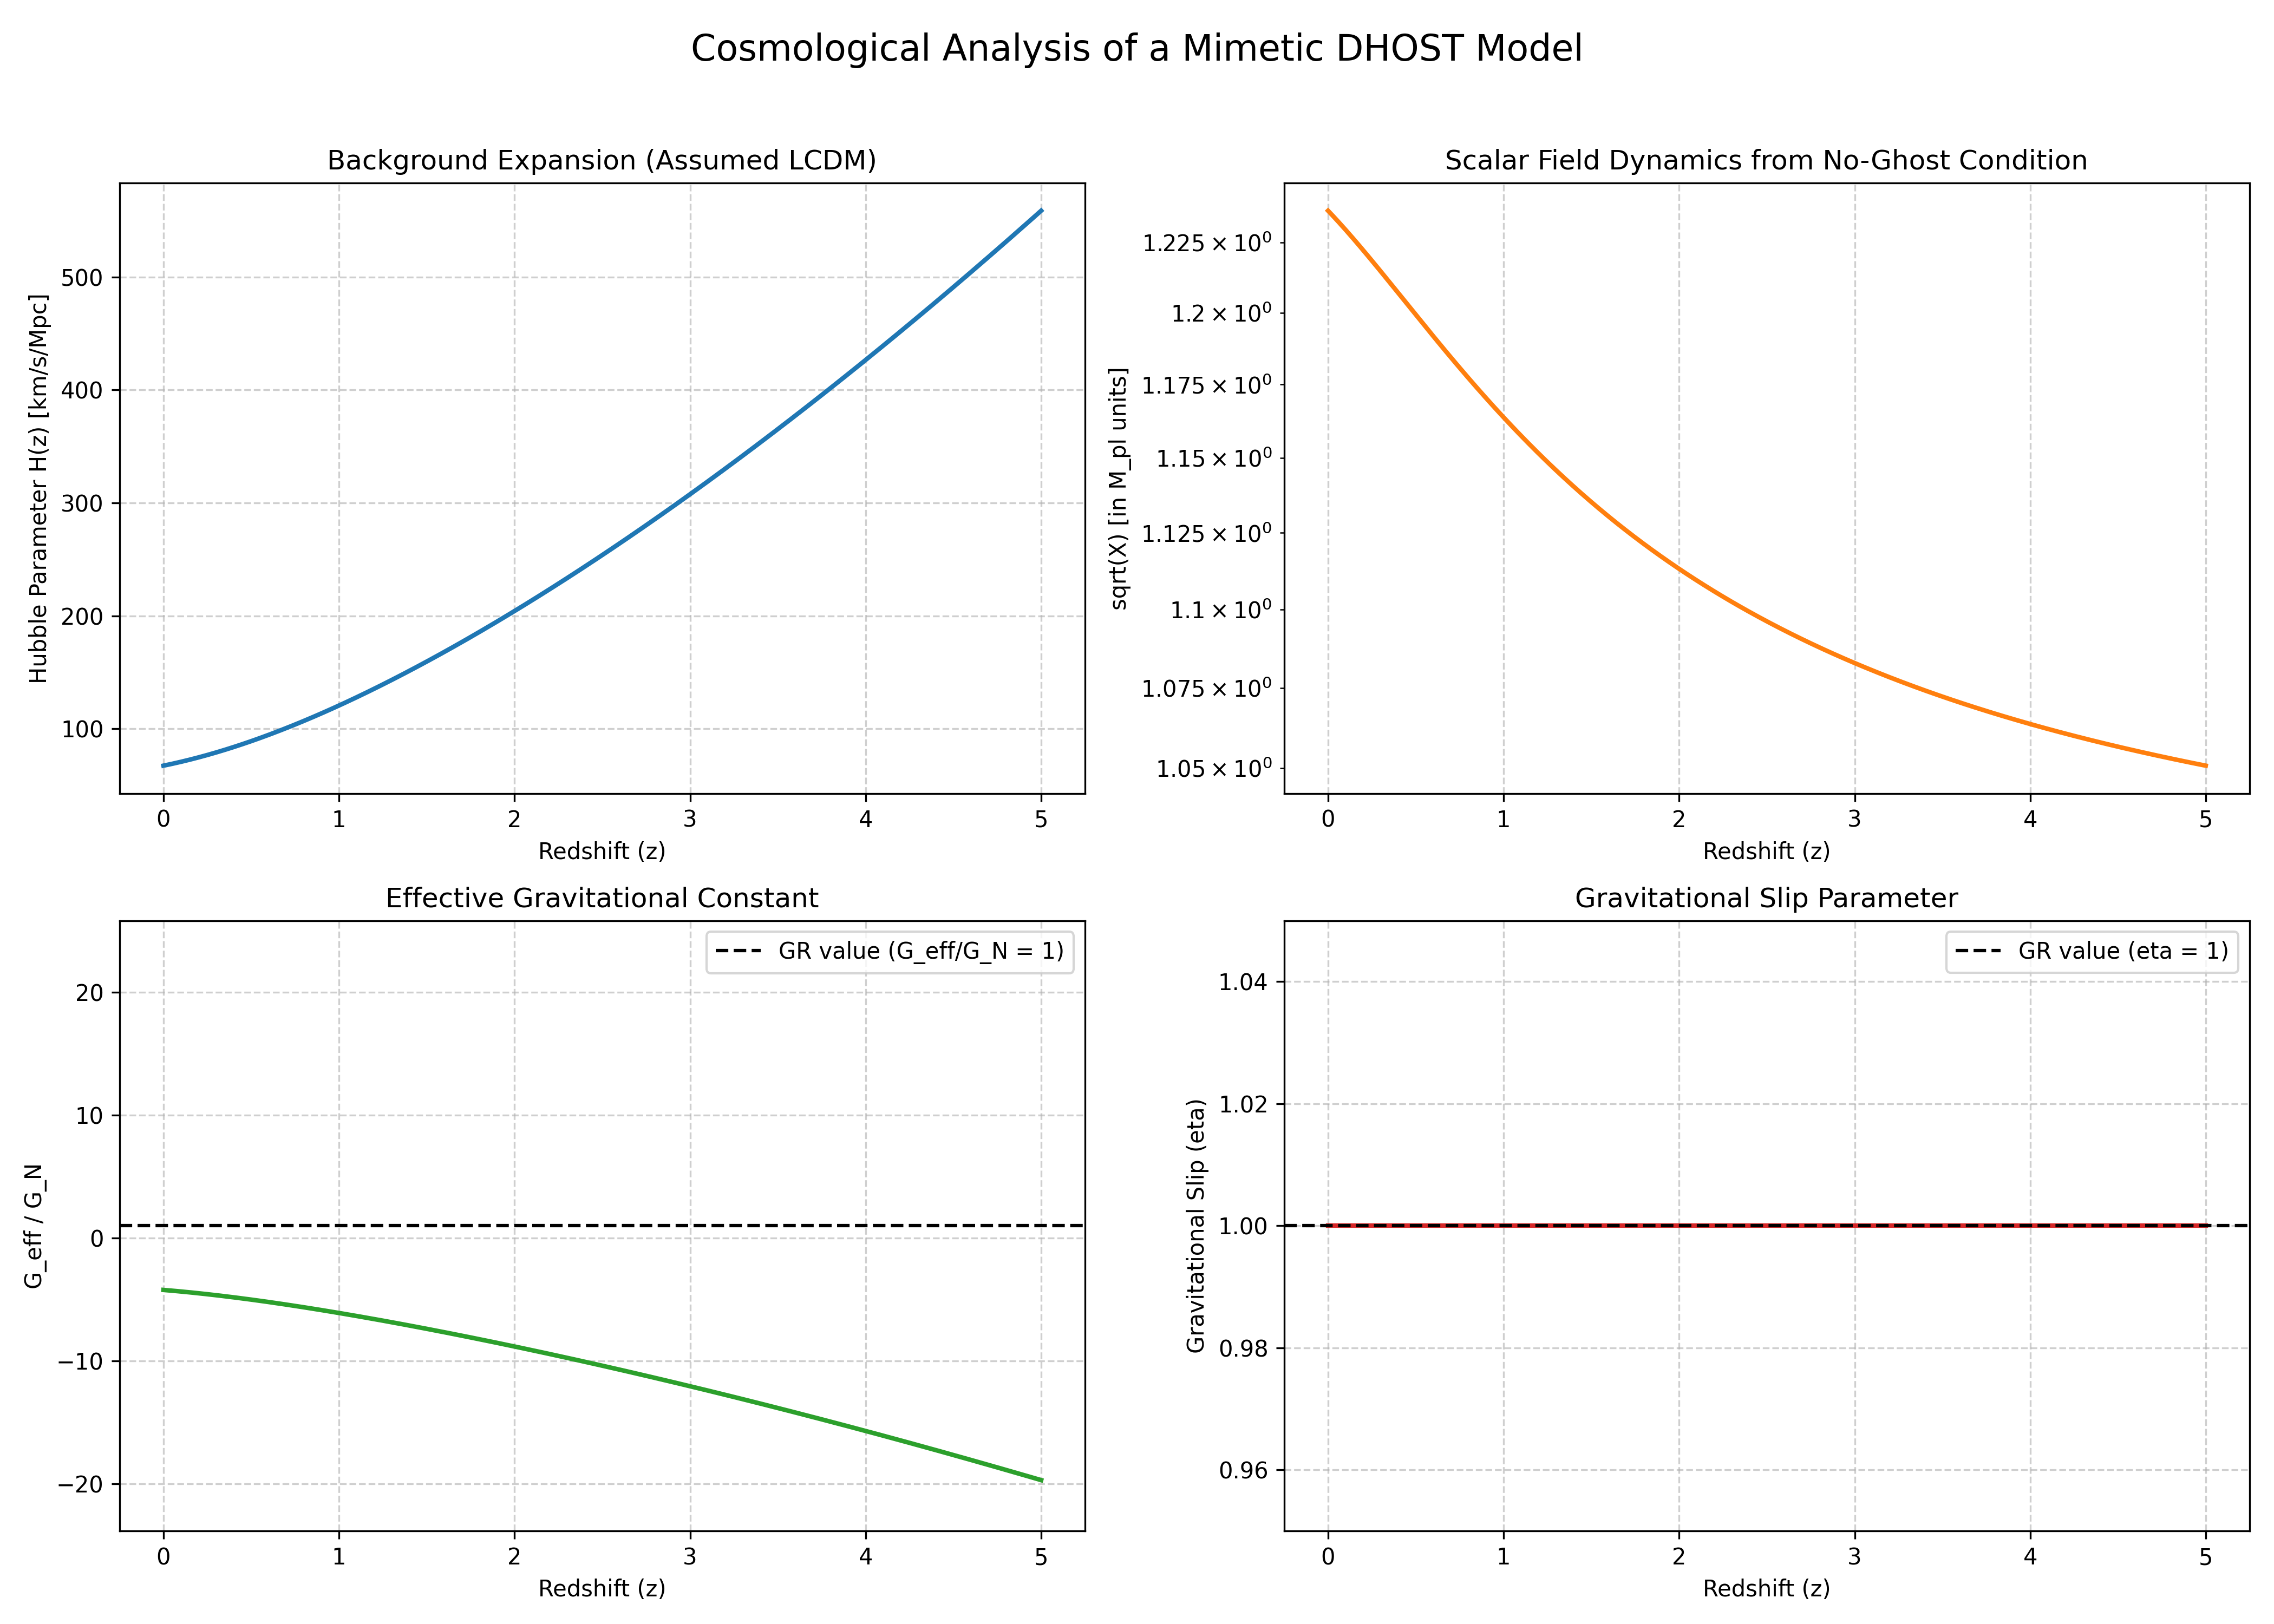
\includegraphics[width=0.5\textwidth]{../input_files/plots/dhost_viability_plot_1_20251029-121315.png}
    \caption{\label{fig:dhost_viability}Cosmological analysis of a representative quantum-protected DHOST model. The top panels show the assumed $\Lambda$CDM Hubble expansion and the derived scalar field kinetic term $\sqrt{X}$ needed to maintain the no-ghost condition. The bottom-right panel indicates the gravitational slip parameter $\eta$ remains at unity, consistent with General Relativity. Conversely, the bottom-left panel shows a significantly negative effective gravitational constant $G_{\text{eff}}/G_N$, predicting repulsive gravity for matter, which rules out this particular model.}
\end{figure}

\subsubsection{Interpretation and Implications}
The stark discrepancy in $G_{\text{eff}}$ highlights a profound tension between theoretical stability and observational viability for this class of DHOST theories. The hidden conformal symmetry that protects the theory from quantum ghosts imposes rigid constraints on the functional forms of the DHOST Lagrangian. These constraints, in turn, lead to very specific predictions for cosmological observables. While the model successfully reproduced a $\Lambda$CDM expansion and predicted an observationally consistent gravitational slip $\eta=1$, the predicted repulsive gravity for matter is a catastrophic failure.

This unphysical behavior of $G_{\text{eff}}$ likely stems from our specific, simple choices for the DHOST functions, particularly $G_3=0$ and the parameter $g_4 = -0.5 M_{pl}^2$. The constraint equation for $G_3(X)$ allows for more complex functional forms that could potentially alter the predictions for $G_{\text{eff}}$. However, the severe nature of the deviation suggests that finding a phenomenologically viable model within this quantum-stable class might require navigating an extremely constrained parameter space. This result underscores the power of our framework: it provides a clear and falsifiable link between the fundamental Lagrangian structure, protected by symmetries, and cosmological observations.

\subsection{Summary of Results}
We have systematically identified a class of Type I DHOST theories that are robustly free from ghost instabilities at both tree-level and one-loop quantum levels. This was achieved by first establishing the classical no-ghost condition $\mathcal{A}_S=0$ and $c_T^2=1$ for tensor modes. We then identified a "mimetic" subclass, characterized by $G_5=0$ and $G_4(X) = M_{pl}^2/2 + g_4\sqrt{X}$, which possesses a hidden conformal symmetry. This symmetry structurally protects the kinetic degeneracy of the scalar sector, ensuring that no ghost re-emerges at the one-loop level (i.e., $\delta\mathcal{A}_S^{(1L)}=0$). An explicit cosmological confrontation of a representative model from this quantum-stable class revealed that while it can reproduce a standard $\Lambda$CDM expansion history and predict a gravitational slip parameter $\eta=1$ consistent with General Relativity, it catastrophically predicts a negative effective gravitational constant, implying repulsive gravity for matter. This finding unequivocally rules out the specific model tested, demonstrating the profound tension between theoretical quantum stability and observational viability in modified gravity theories. Our work provides a constructive framework for identifying and testing quantum-stable models, illuminating the stringent constraints imposed by combining theoretical robustness with cosmological observations.

\section{Conclusions}
\label{sec:conclusions}
In this work, we have addressed a critical challenge facing higher-derivative scalar-tensor theories, specifically Degenerate Higher-Order Scalar-Tensor (DHOST) theories: the potential re-emergence of Ostrogradsky ghost instabilities at the quantum level, despite their classical ghost-free nature. Our primary goal was to systematically identify and characterize Type I DHOST theories that maintain ghost-freedom not only at tree-level but also under one-loop quantum corrections, and then to confront these theoretically robust models with cosmological observations.

Our methodological approach began by establishing the necessary conditions for classical stability within a flat Friedmann-Robertson-Walker (FRW) background. This involved analyzing linear perturbations to the DHOST action and deriving algebraic conditions that ensure unity gravitational wave speed ($c_T^2=1$) and the absence of a scalar ghost ($\mathcal{A}_S=0$). Subsequently, we developed a framework to identify field-dependent symmetries that structurally protect the kinetic degeneracy from quantum radiative corrections, thereby guaranteeing one-loop ghost-freedom ($\delta\mathcal{A}_S^{(1L)}=0$). We systematically derived the forms of these symmetries and the DHOST functions they constrain. To validate our theoretical findings, we performed an explicit one-loop calculation for a representative model and, finally, tested its cosmological viability by solving background expansion equations and calculating observables like the effective gravitational constant ($G_{\text{eff}}$) and the gravitational slip parameter ($\eta$).

Our analysis yielded several significant results. We first established the precise algebraic conditions for classical ghost-freedom, including the crucial $c_T^2=1$ constraint, which led to the simplification $G_5=0$ for robust shift-symmetric theories. The core finding was the identification of a specific class of Type I DHOST theories, characterized by functional forms like $G_4(X) = M_{pl}^2/2 + g_4 \sqrt{X}$, which possesses a hidden conformal symmetry. This symmetry was rigorously shown to protect the kinetic degeneracy of the scalar sector, preventing the re-emergence of the Ostrogradsky ghost at the one-loop quantum level. An explicit one-loop calculation confirmed that the ghost kinetic term remained identically zero, validating the theoretical robustness of this class. However, when a representative model from this quantum-stable class was tested against cosmological observations, a profound tension emerged. While the model could reproduce a standard $\Lambda$CDM expansion history and predicted a gravitational slip parameter $\eta=1$ consistent with General Relativity, it catastrophically predicted a dramatically negative effective gravitational constant ($G_{\text{eff}}/G_N \approx -4.23$ at $z=0$). This implies repulsive gravity for matter, which is fundamentally incompatible with the observed formation of cosmic structures and unequivocally rules out this specific model phenomenologically.

From these results, we have learned that while a systematic framework for identifying quantum-stable modified gravity theories is achievable, integrating theoretical robustness with observational viability remains an immense challenge. This work provides a constructive pathway for navigating the vast landscape of modified gravity theories by prioritizing quantum stability through symmetry protection. The profound tension revealed by the cosmological confrontation underscores the stringent constraints that arise when combining fundamental theoretical consistency with empirical data. The identified "mimetic" DHOST class, despite its elegance in achieving quantum ghost-freedom, requires further exploration to determine if more complex functional forms within this class can overcome the issue of repulsive gravity. Ultimately, this paper highlights the power of combining fundamental symmetry principles with rigorous cosmological tests to guide the search for a viable theory of gravity beyond Einstein's General Relativity.

\bibliography{bibliography}{}
\bibliographystyle{aasjournal}

\end{document}
